\chapter{L1's effect on phonetic properties of accented speech}
\label{l1_seg}

\section{Introduction}

This section will investigate the statistical relationship between the phonetic acoustic measurements extracted from accented American English speech (independent variables) and the perceived accetendenss score provided by native American English speakers (dependent variables). Two sets of features will be used as independent variables: one is the pronunciation score based features extracted only using L2 acoustic model and the other one is the pronunciation score based features extracted using both L1 and L2 acoustic model. This corresponds to the data analysis 1 in figure \ref{fig:method_diagram} using only L2 normalized segmental acoustic measurements and the combination of  both L1 and L2 normalized segmental acoustic measurements. First, correlational relationship between independent variables and dependent variables. Second, multiple regression analysis will be employed to analyze how well each set of features can predict the accentedness score. Results and discussion are in the final part.

\section{Methods}


For each foreign language, the correlation analysis will be done between each dimension of the feature vector and the accentedness scores ( average of all 13 annotators). The correlation analysis is done L1 independently in hope that some L1 specific information will be revealed. The Spearman correlation coefficients and the corresponding p-value for testing non-correlation will be calculated in this part. Higher correlation coefficients means better correlation and lower p-value means correlation is more significant.

\begin{figure}[t]
        \begin{minipage}[t]{1\linewidth}
        \centering
            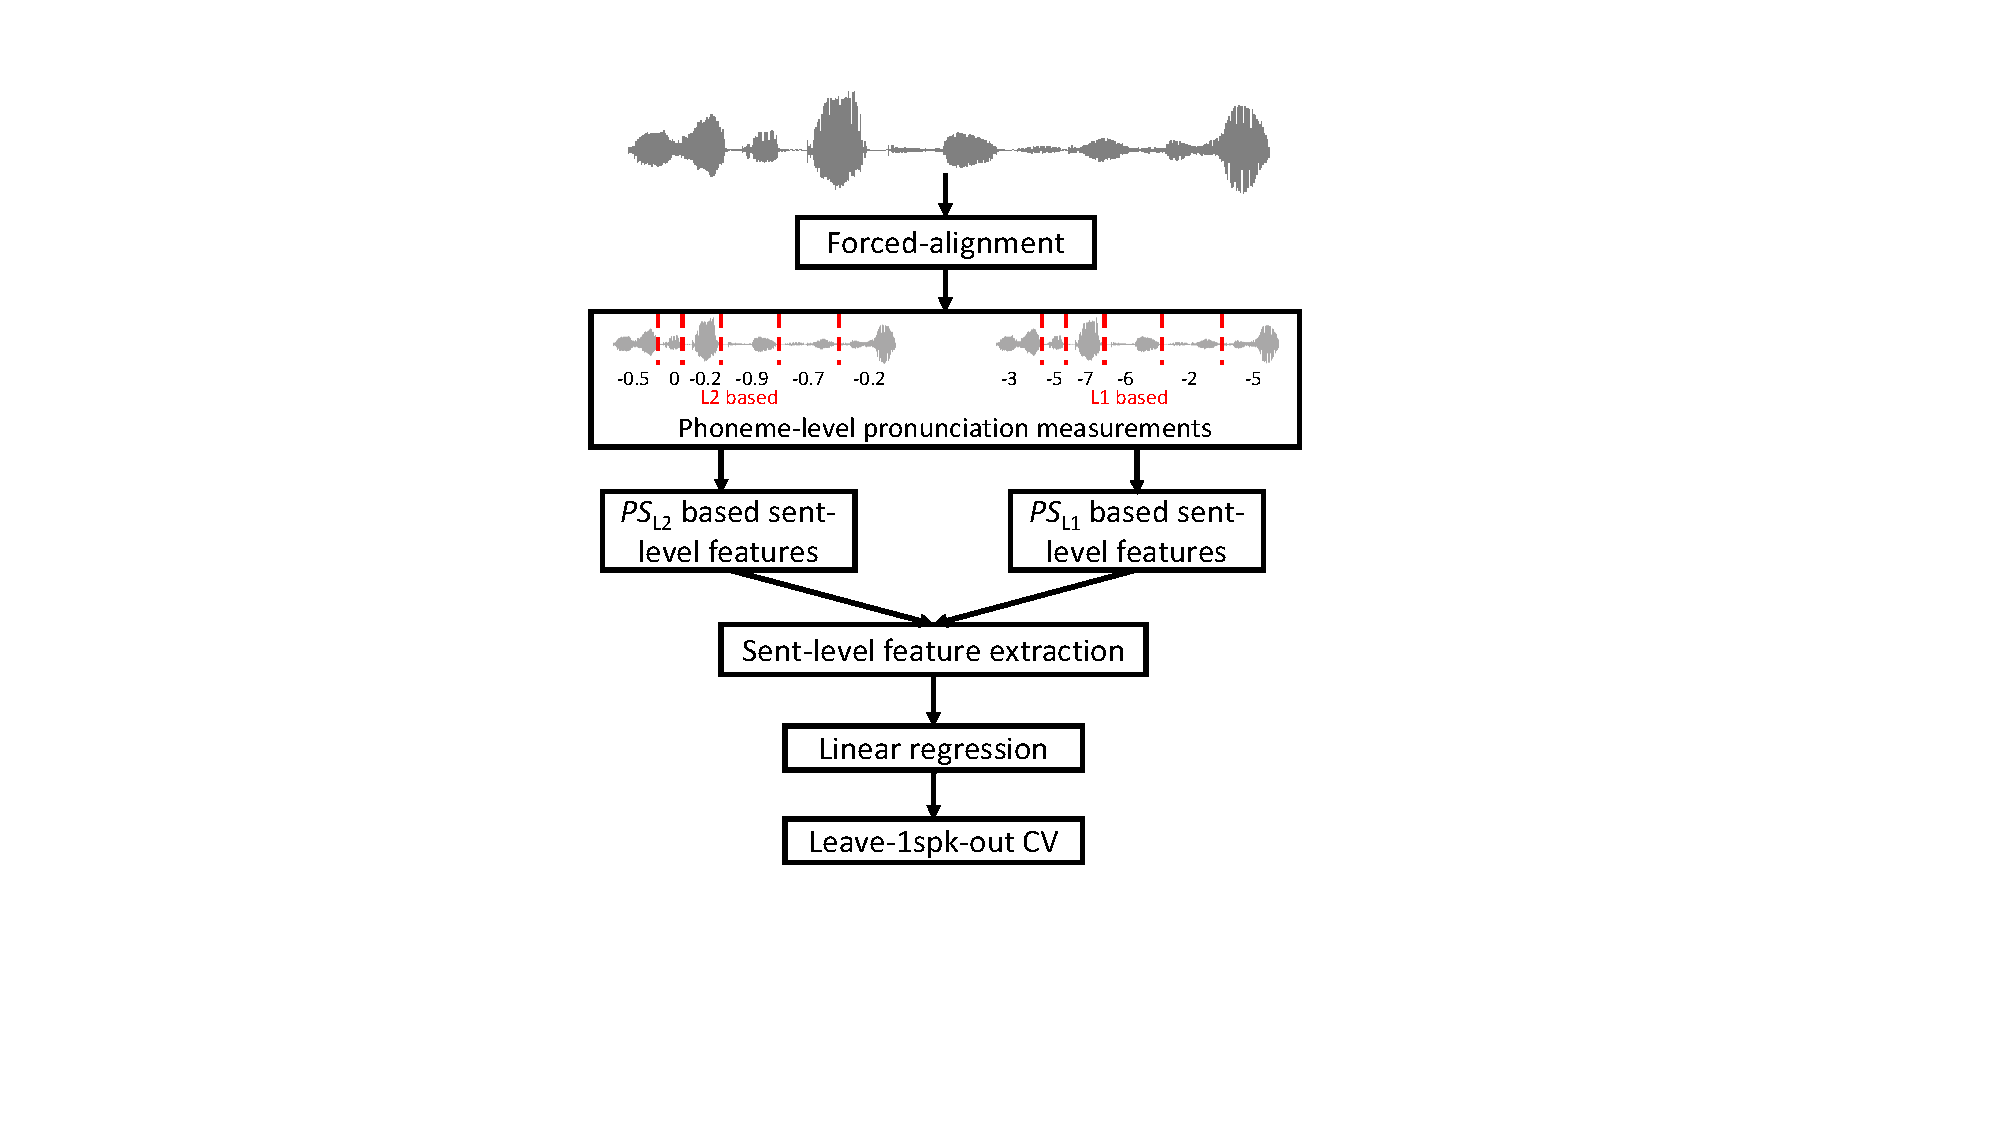
\includegraphics[width=3.0in]{figures/L1_seg_diagram.pdf}
        \end{minipage}%
        \caption{Diagram of the procedure for multiple regression analysis between pronunciation based acoustic measurements and accentedness score.}
        \centering
        \label{fig:l1_seg_diagram}
     \end{figure}

The whole procedure of multiple regression analysis is shown in figure \ref{fig:l1_seg_diagram}. The upper part of the figure shows the feature extraction scheme in section \ref{sec:segmental} and will not be described here. Each speaker had a 12-dimensional feature vector quantifying how close their pronunciation is to L2 and another 12-dimensional feature vector quantifying how close their pronunciation is to their L1.. After extracting utterance-level features for all speakers, each speaker has a feature vector and a corresponding accentedness score (in the range of 1 to 4). For speakers that belong to the same L1 category, a linear regression model with an L2 norm regularizer (or ridge regression) is built with data from 29 speakers used to train the model and the remaining speaker used to evaluate the model. The feature vectors were mean and variance normalized first. Feature selection based on univariate linear regression test \citep{saeys2007review} was also used to select the most predictable features. Basically, the feature selector calculates a score (based on the correlation coefficients between independent variables and dependent variables) for each independent variables given labels in training set and select the independent variables with highest scores. The scikit-learn toolkit was used to implement feature normalization, feature selection and ridge regression \citep{scikit-learn}. To generate the accentedness prediction for all speakers, evaluation using leave-one-speaker-out CV was performed; this means that a feature selector and a ridge regression model is trained on all combinations of 29 speakers out of 30 speakers and tested on the 1 remaining. For different input features (12-dimensional utterance-level features or 24-dimensional utterance-level features), the hyperparameters were tuned to achieve the best performance.

As mentioned in section \ref{sec:data_collection}, the accentedness label distributions for German and French speakers do not span the 1-4 rating scale uniformly. The initial result revealed that the model performance on German and French speakers was comparatively lower (but there was still improvement by adding the feature vector extracted using L1 acoustic model). In an attempt to train our model with more uniformly distributed labels, the German speakers were randomly downsampled from 30 to 18 and French speakers from 30 to 22 in an attempt to uniformly sample the labels. For other two languages, there are still 30 speakers in the results. The Pearson correlation coefficient (PCC, higher better) and the mean absolute error (MAE, lower better) are used to measure the relationship between model prediction and human scores.

\section{Results}

\subsection{Results of correlation analysis}

\begin{table}[]
\centering
\caption{Pearson correlation coefficients (first line) together with p-value (second line) between acoustic measurements extracted from L1 and l2 acoustic models and accentedness scores of four different foreign languages.}
\label{table:seg_corr}
\resizebox{\columnwidth}{!}{%
\begin{tabular}{|c|c|c|c|c|c|c|c|c|}
\hline
 & \multicolumn{4}{c|}{Based on L2 AM} & \multicolumn{4}{c|}{Based on L1 AM} \\ \hline
 & German & French & Mandarin & Spanish & German & French & Mandarin & Spanish \\ \hline
\begin{tabular}[c]{@{}c@{}}Minimum of \\ vowels' PS\end{tabular} & \begin{tabular}[c]{@{}c@{}}-0.00\\ 9.84E-01\end{tabular} & \begin{tabular}[c]{@{}c@{}}-0.05\\ 7.90E-01\end{tabular} & \begin{tabular}[c]{@{}c@{}}-0.53\\ 2.78E-03\end{tabular} & \begin{tabular}[c]{@{}c@{}}-0.17\\ 3.58E-01\end{tabular} & \begin{tabular}[c]{@{}c@{}}0.12\\ 5.11E-01\end{tabular} & \begin{tabular}[c]{@{}c@{}}0.09\\ 6.43E-01\end{tabular} & \begin{tabular}[c]{@{}c@{}}0.12\\ 5.27E-01\end{tabular} & \begin{tabular}[c]{@{}c@{}}0.35\\ 5.89E-02\end{tabular} \\ \hline
\begin{tabular}[c]{@{}c@{}}Minimum of \\ consonants' PS\end{tabular} & \begin{tabular}[c]{@{}c@{}}-0.24\\ 1.95E-01\end{tabular} & \begin{tabular}[c]{@{}c@{}}-0.15\\ 4.33E-01\end{tabular} & \begin{tabular}[c]{@{}c@{}}-0.11\\ 5.69E-01\end{tabular} & \begin{tabular}[c]{@{}c@{}}-0.47\\ 9.26E-03\end{tabular} & \textbf{\begin{tabular}[c]{@{}c@{}}-0.15\\ 4.36E-01\end{tabular}} & \begin{tabular}[c]{@{}c@{}}0.34\\ 6.80E-02\end{tabular} & \begin{tabular}[c]{@{}c@{}}-0.03\\ 8.82E-01\end{tabular} & \begin{tabular}[c]{@{}c@{}}0.07\\ 7.30E-01\end{tabular} \\ \hline
\begin{tabular}[c]{@{}c@{}}Minimum of \\ syllables' PS\end{tabular} & \begin{tabular}[c]{@{}c@{}}0.00\\ 9.83E-01\end{tabular} & \begin{tabular}[c]{@{}c@{}}-0.05\\ 7.85E-01\end{tabular} & \begin{tabular}[c]{@{}c@{}}-0.33\\ 7.69E-02\end{tabular} & \begin{tabular}[c]{@{}c@{}}-0.20\\ 2.82E-01\end{tabular} & \begin{tabular}[c]{@{}c@{}}-0.01\\ 9.50E-01\end{tabular} & \begin{tabular}[c]{@{}c@{}}0.24\\ 2.08E-1\end{tabular} & \begin{tabular}[c]{@{}c@{}}0.31\\ 9.80E-02\end{tabular} & \begin{tabular}[c]{@{}c@{}}0.20\\ 2.98E-01\end{tabular} \\ \hline
\begin{tabular}[c]{@{}c@{}}Average of \\ vowels' PS\end{tabular} & \begin{tabular}[c]{@{}c@{}}-0.23\\ 2.31E-01\end{tabular} & \begin{tabular}[c]{@{}c@{}}-0.43\\ 1.75E-02\end{tabular} & \begin{tabular}[c]{@{}c@{}}-0.64\\ 1.43E-04\end{tabular} & \textbf{\begin{tabular}[c]{@{}c@{}}-0.69\\ 2.21E-05\end{tabular}} & \begin{tabular}[c]{@{}c@{}}-0.10\\ 5.85E-01\end{tabular} & \begin{tabular}[c]{@{}c@{}}0.28\\ 1.39E-01\end{tabular} & \begin{tabular}[c]{@{}c@{}}0.55\\ 1.52E-03\end{tabular} & \textbf{\begin{tabular}[c]{@{}c@{}}0.53\\ 2.68E-03\end{tabular}} \\ \hline
\begin{tabular}[c]{@{}c@{}}Average of \\ consonants' PS\end{tabular} & \textbf{\begin{tabular}[c]{@{}c@{}}-0.41\\ 2.54E-02\end{tabular}} & \begin{tabular}[c]{@{}c@{}}-0.33\\ 7.95E-02\end{tabular} & \begin{tabular}[c]{@{}c@{}}-0.64\\ 1.40E-04\end{tabular} & \textbf{\begin{tabular}[c]{@{}c@{}}-0.69\\ 2.08E-05\end{tabular}} & \begin{tabular}[c]{@{}c@{}}0.06\\ 7.63E-01\end{tabular} & \textbf{\begin{tabular}[c]{@{}c@{}}0.56\\ 1.45E-03\end{tabular}} & \begin{tabular}[c]{@{}c@{}}0.33\\ 7.18E-02\end{tabular} & \begin{tabular}[c]{@{}c@{}}0.31\\ 9.56E-02\end{tabular} \\ \hline
\begin{tabular}[c]{@{}c@{}}Average of \\ syllables' PS\end{tabular} & \begin{tabular}[c]{@{}c@{}}-0.33\\ 7.08E-02\end{tabular} & \begin{tabular}[c]{@{}c@{}}-0.36\\ 4.07E-02\end{tabular} & \begin{tabular}[c]{@{}c@{}}-0.68\\ 3.07E-05\end{tabular} & \begin{tabular}[c]{@{}c@{}}-0.68\\ 2.86E-05\end{tabular} & \begin{tabular}[c]{@{}c@{}}0.00\\ 9.96E-01\end{tabular} & \begin{tabular}[c]{@{}c@{}}0.48\\ 6.70E-03\end{tabular} & \textbf{\begin{tabular}[c]{@{}c@{}}0.56\\ 1.17E-03\end{tabular}} & \begin{tabular}[c]{@{}c@{}}0.44\\ 1.40E-02\end{tabular} \\ \hline
\begin{tabular}[c]{@{}c@{}}STD of \\ vowels' PS\end{tabular} & \begin{tabular}[c]{@{}c@{}}0.17\\ 3.73E-01\end{tabular} & \begin{tabular}[c]{@{}c@{}}0.14\\ 4.65E-01\end{tabular} & \begin{tabular}[c]{@{}c@{}}0.61\\ 2.76E-04\end{tabular} & \begin{tabular}[c]{@{}c@{}}0.43\\ 1.62E-02\end{tabular} & \begin{tabular}[c]{@{}c@{}}-0.06\\ 7.52E-01\end{tabular} & \begin{tabular}[c]{@{}c@{}}-0.32\\ 8.22E-02\end{tabular} & \begin{tabular}[c]{@{}c@{}}-0.47\\ 9.05E-03\end{tabular} & \begin{tabular}[c]{@{}c@{}}-0.31\\ 9.40E-02\end{tabular} \\ \hline
\begin{tabular}[c]{@{}c@{}}STD of \\ consonants' PS\end{tabular} & \begin{tabular}[c]{@{}c@{}}0.26\\ 1.61E-01\end{tabular} & \begin{tabular}[c]{@{}c@{}}0.22\\ 2.38E-01\end{tabular} & \begin{tabular}[c]{@{}c@{}}0.40\\ 3.05E-02\end{tabular} & \begin{tabular}[c]{@{}c@{}}0.61\\ 3.45E-04\end{tabular} & \begin{tabular}[c]{@{}c@{}}-0.07\\ 7.24E-01\end{tabular} & \begin{tabular}[c]{@{}c@{}}-0.19\\ 3.10E-01\end{tabular} & \begin{tabular}[c]{@{}c@{}}0.38\\ 4.00E-02\end{tabular} & \begin{tabular}[c]{@{}c@{}}-0.16\\ 3.88E-01\end{tabular} \\ \hline
\begin{tabular}[c]{@{}c@{}}STD of \\ syllables' PS\end{tabular} & \begin{tabular}[c]{@{}c@{}}0.16\\ 4.04E-01\end{tabular} & \begin{tabular}[c]{@{}c@{}}0.12\\ 5.41E-01\end{tabular} & \begin{tabular}[c]{@{}c@{}}0.43\\ 1.87E-02\end{tabular} & \begin{tabular}[c]{@{}c@{}}0.34\\ 6.48E-02\end{tabular} & \begin{tabular}[c]{@{}c@{}}-0.07\\ 7.04E-01\end{tabular} & \begin{tabular}[c]{@{}c@{}}-0.38\\ 3.95E-02\end{tabular} & \begin{tabular}[c]{@{}c@{}}-0.10\\ 5.94E-01\end{tabular} & \textbf{\begin{tabular}[c]{@{}c@{}}-0.53\\ 2.49E-03\end{tabular}} \\ \hline
\begin{tabular}[c]{@{}c@{}}STD\_norm of \\ vowels' PS\end{tabular} & \begin{tabular}[c]{@{}c@{}}0.29\\ 1.22E-01\end{tabular} & \textbf{\begin{tabular}[c]{@{}c@{}}0.49\\ 6.36E-03\end{tabular}} & \begin{tabular}[c]{@{}c@{}}0.36\\ 5.30E-02\end{tabular} & \begin{tabular}[c]{@{}c@{}}0.52\\ 2.97E-03\end{tabular} & \begin{tabular}[c]{@{}c@{}}0.12\\ 5.44E-01\end{tabular} & \begin{tabular}[c]{@{}c@{}}0.11\\ 5.51E-01\end{tabular} & \begin{tabular}[c]{@{}c@{}}-0.22\\ 2.35E-01\end{tabular} & \begin{tabular}[c]{@{}c@{}}-0.23\\ 2.20E-01\end{tabular} \\ \hline
\begin{tabular}[c]{@{}c@{}}STD\_norm of \\ consonants' PS\end{tabular} & \begin{tabular}[c]{@{}c@{}}0.33\\ 7.56E-02\end{tabular} & \begin{tabular}[c]{@{}c@{}}0.32\\ 8.90E-02\end{tabular} & \textbf{\begin{tabular}[c]{@{}c@{}}0.73\\ 4.97E-06\end{tabular}} & \begin{tabular}[c]{@{}c@{}}0.56\\ 1.22E-03\end{tabular} & \begin{tabular}[c]{@{}c@{}}0.06\\ 7.64E-01\end{tabular} & \begin{tabular}[c]{@{}c@{}}-0.07\\ 6.94E-1\end{tabular} & \begin{tabular}[c]{@{}c@{}}-0.44\\ 1.54E-02\end{tabular} & \begin{tabular}[c]{@{}c@{}}-0.01\\ 9.73E-01\end{tabular} \\ \hline
\begin{tabular}[c]{@{}c@{}}STD\_norm of \\ syllables' PS\end{tabular} & \begin{tabular}[c]{@{}c@{}}0.39\\ 3.51E-02\end{tabular} & \begin{tabular}[c]{@{}c@{}}0.42\\ 1.96E-02\end{tabular} & \begin{tabular}[c]{@{}c@{}}0.69\\ 2.82E-05\end{tabular} & \begin{tabular}[c]{@{}c@{}}0.57\\ 9.85E-04\end{tabular} & \begin{tabular}[c]{@{}c@{}}0.09\\ 6.48E-01\end{tabular} & \begin{tabular}[c]{@{}c@{}}0.23\\ 2.27E-01\end{tabular} & \begin{tabular}[c]{@{}c@{}}-0.33\\ 7.26E-02\end{tabular} & \begin{tabular}[c]{@{}c@{}}0.21\\ 2.63E-01\end{tabular} \\ \hline
\end{tabular}
}
\end{table}

In table \ref{table:seg_corr}, PCC (first line) together with p-value (second line) between acoustic measurements extracted from L1 and l2 acoustic models and accentedness scores of four different foreign languages are presented. In the table, ``AM'' is short for ``acoustic model''; ``PS'' is short for ``pronunciation score''; ``STD'' is short for ``Standard deviation''; ``STD\_norm'' is short for ``mean normalized standard deviation''. For each feature set (based on L2 AM or based on L1 AM), the highest correlation between each feature and accentedness score is in bold for all four foreign languages. From the table, there are several interesting observations:

\begin{figure}[t]
        \begin{minipage}[t]{0.5\linewidth}
        \centering
            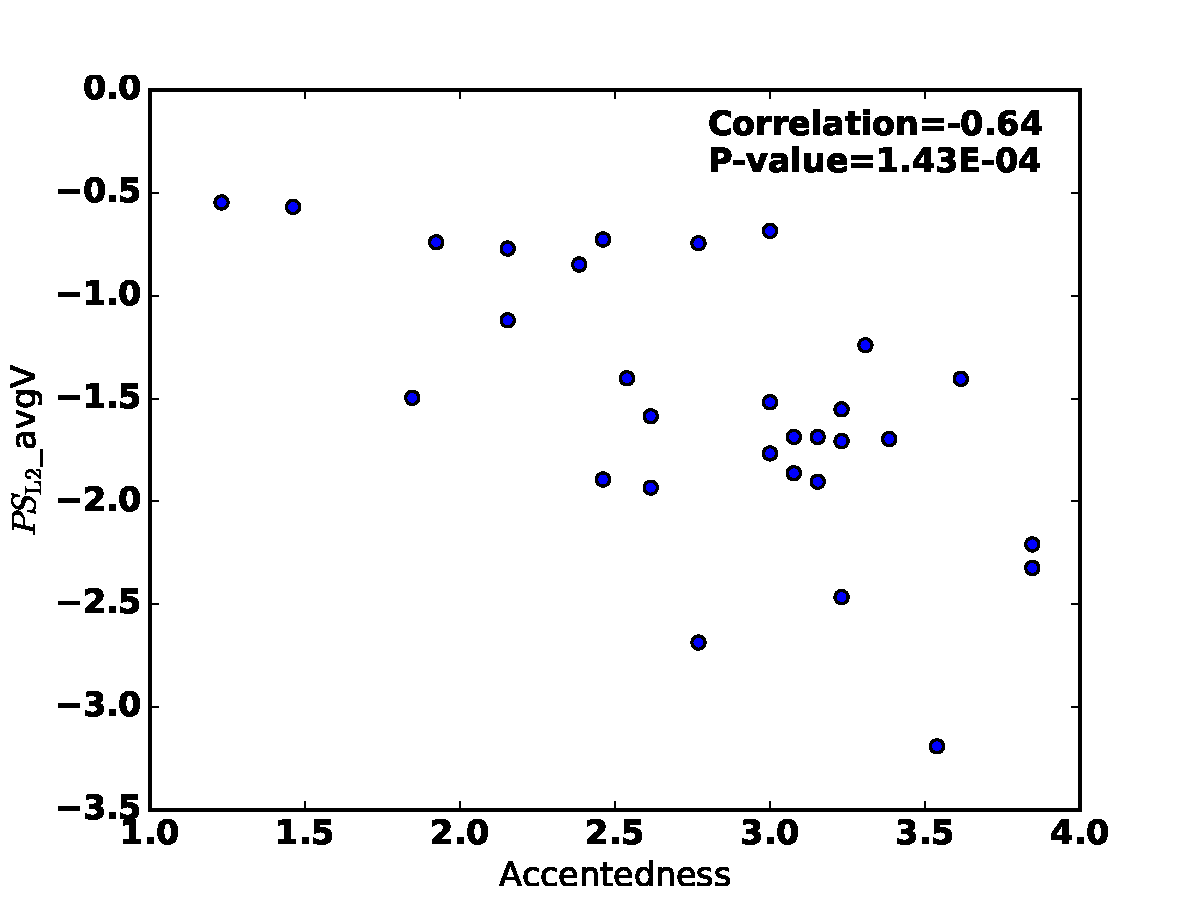
\includegraphics[width=3in]{figures/seg_scatter/figure2_1.pdf}
        \end{minipage}%
        \begin{minipage}[t]{0.5\linewidth}
        \centering
            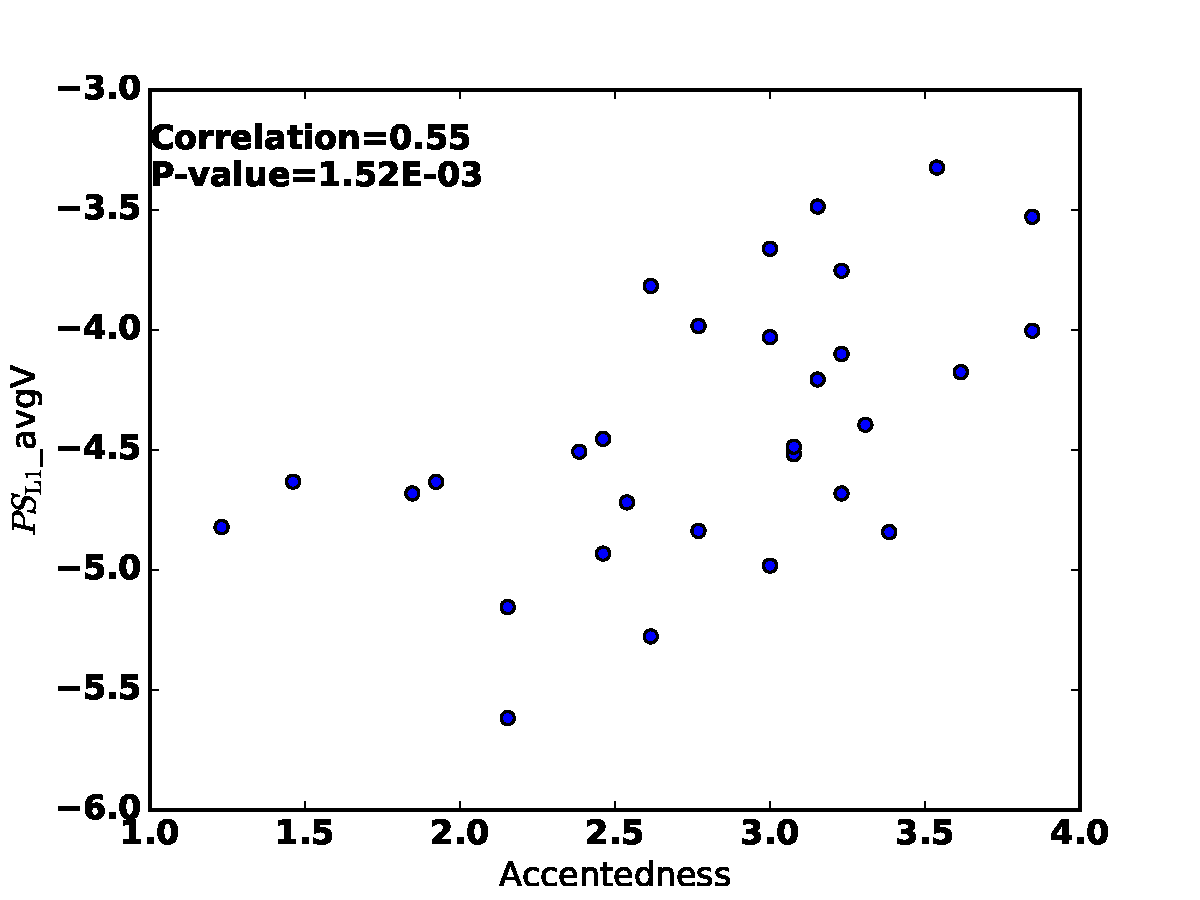
\includegraphics[width=3in]{figures/seg_scatter/figure2_2.pdf}
        \end{minipage}%
        \\
        \begin{minipage}[t]{0.5\linewidth}
        \centering
            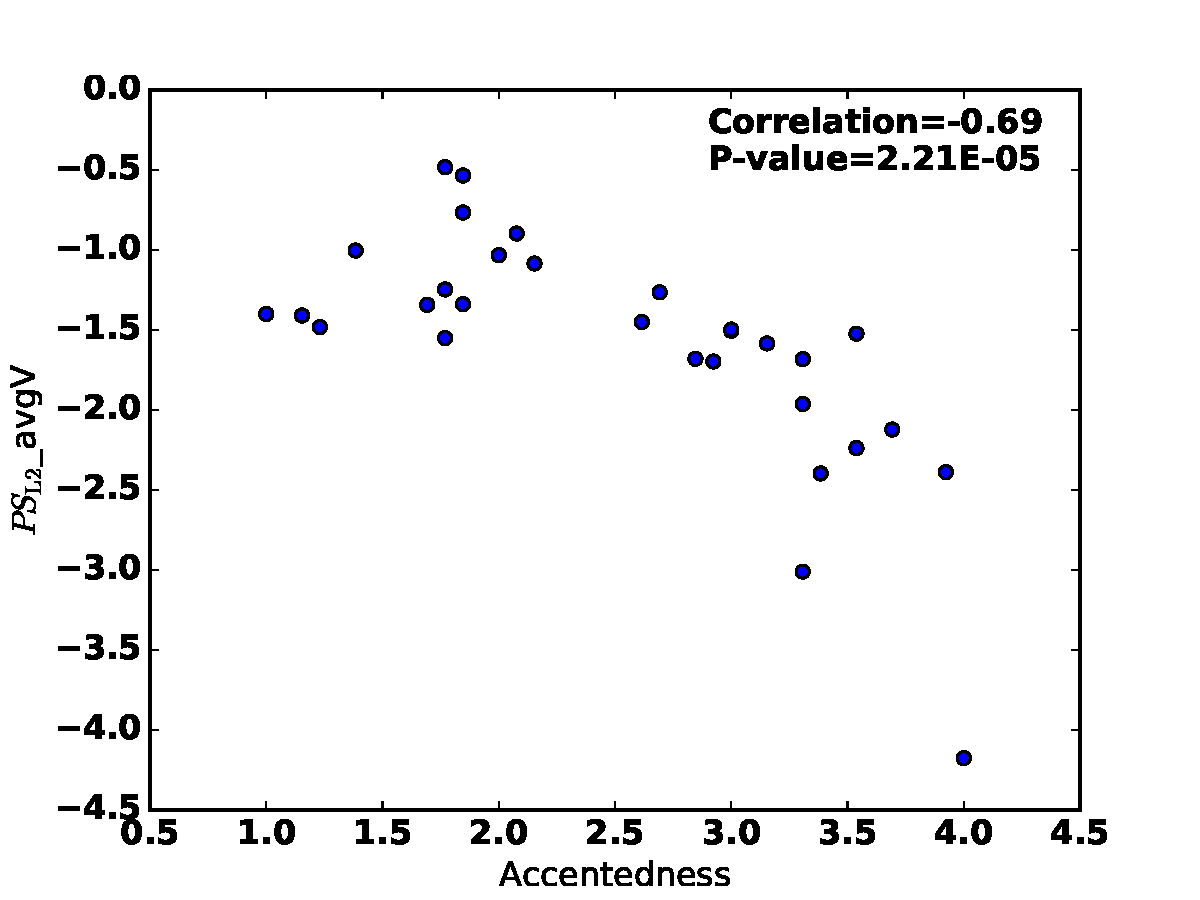
\includegraphics[width=3in]{figures/seg_scatter/figure2_3.pdf}
        \end{minipage}%
        \begin{minipage}[t]{0.5\linewidth}
        \centering
            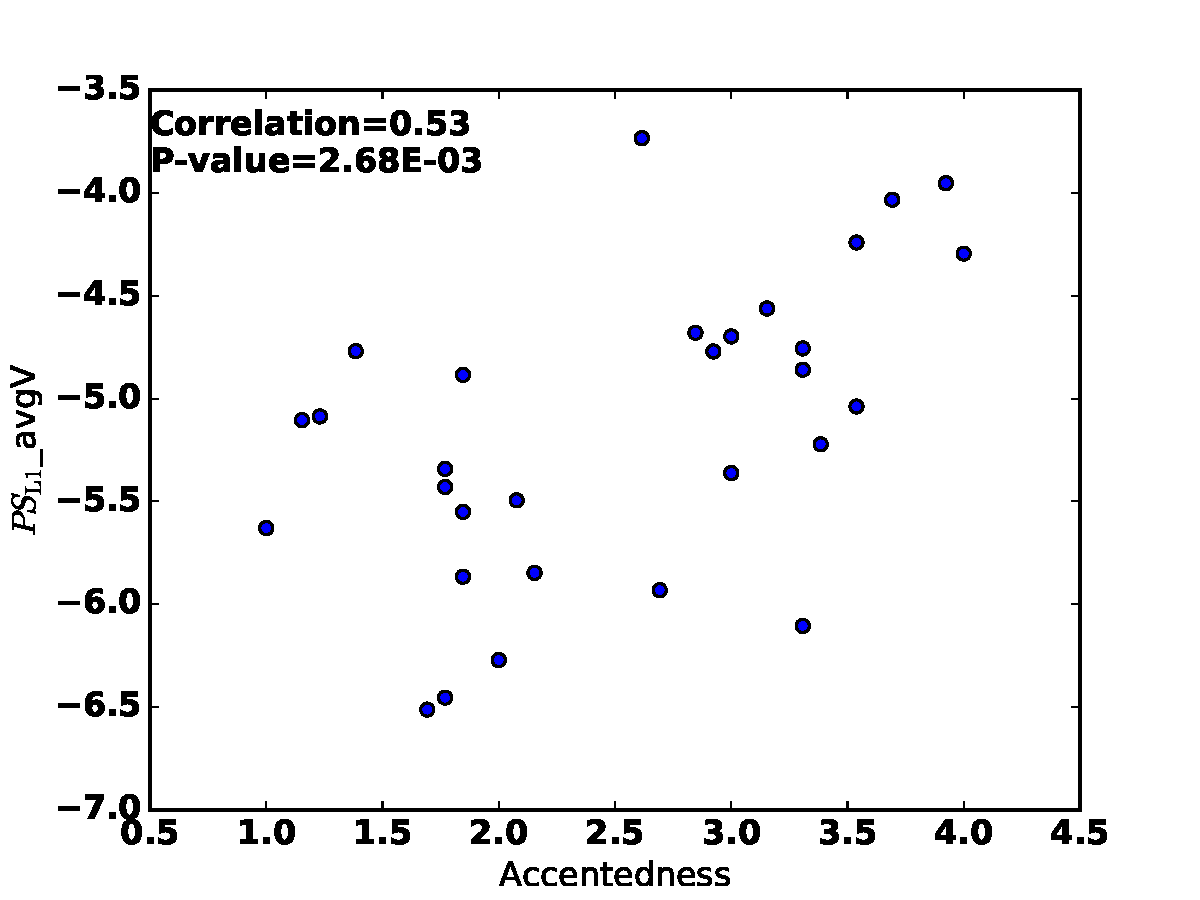
\includegraphics[width=3in]{figures/seg_scatter/figure2_4.pdf}
        \end{minipage}%
        \caption{Scatter plots between accentedness scores and one dimension of features for Mandarin (first row) and Spanish (second row) speakers.}
        \centering
        \label{fig:seg_scatter}
     \end{figure}

\begin{enumerate}
 \item For minimum and average features (row 3 to row 8), the correlations with low p-value (means significantly correlated) achieved with L2 acoustic model are negative while those achieved with l1 acoustic model are positive. This can be interpreted with the physical meanings of the two feature sets. As introduced in section \ref{sec:segmental}, for these pronunciation score based features, higher value means closer to pronunciation patterns model by corresponding acoustic models. Thus, for minimum and average features extracted with L1 acoustic model, higher value means the pronunciation of English is closer to pronunciation patterns of the L1; If a speaker is using the pronunciation patterns of his L1 to produce English, very possibly he has a high accentedness score (towards 4 on the scale); Thus, the correlation coefficients between minimum and average features and accentedness scores are positive. On the contrary, for minimum and average features extracted with L2 English acoustic model, higher value means the pronunciation with accent is closer to pronunciation patterns of native English speakers; Thus, the correlation coefficients are negative. In most cases, the correlation coefficients of minimum features are relatively low while the correlation coefficients of average features are relatively high, which tells that the accentedness score can not be determined by one or two very low pronunciation scores.
 \item For STD features (row 9 to row 11), the patterns are on the other side compared to minimum and average features. This is also easy to interpret: higher STD means there are some very low pronunciation scores; In terms of features extracted with L2 acoustic models, this means possibly higher accentedness score; In terms of features extracted with L1 acoustic models, this means possible lower accentedness score. The correlation coefficients of STD features are also relatively low compared to average features.
 \item STD\_norm features (row 12 to row 14) extracted with L1 acoustic model are not very correlative with accentedness score. However, those extracted with L2 acoustic models can have very high correlation coefficients (such as Mandarin speakers). STD\_norm features are calculated by dividing values of STD features with values of average features. Ideally, it should have same correlational pattern with STD features considering average features and STD features are oppositely correlated with accentedness score.
 \item While the features achieved with L2 acoustic models have higher correlation coefficients with accentedness score, features extracted with L1 acoustic models also show high correlations. This partly support the hypothesis in chapter \ref{introduction} that ``the phonological distance between accented speech and speaker's L1 are negatively correlated with perceived accentedness;''. In figure \ref{fig:seg_scatter}, the scatter plots between average of vowels' PS and accentedness score are presented for Mandarin and Spanish speakers. Based on this observation, it is more likely that when combining features extracted with both L1 and L2 acoustic models can better fit the accentedness score.
\end{enumerate}

\subsection{Results of multiple regression analysis}

In table \ref{table:seg_pred}, both the PCCs and MAEs between model predicted accentedness and human annotated accentedness for 4 groups of speakers are presented. The results of German and French speakers before down-sampling are also showed in the parentheses. There is a clear improvement when adding L1 acoustic model based features for all 4 L1s. These results show that there is an improvement in model performance consistently and across all languages after adding features from the L1 acoustic model. It proves that the L1 contrastive information between accented speech and L1 can provide extra information for accentedness prediction. This is despite the fact that the annotators know little about the acoustic properties of the speakers' L1s.

\begin{table}[t]
\centering
\caption{PCCs and MAEs between predicted accentedness and human scores for speakers of 4 different L1s.}
\label{table:seg_pred}
\begin{tabular}{|c|c|c|c|c|}
\hline
\multirow{2}{*}{} & \multicolumn{2}{c|}{$PS_{\mathrm{L2}}$ only} & \multicolumn{2}{c|}{$PS_{\mathrm{L2}}$ and $PS_{\mathrm{L1}}$} \\ \cline{2-5}
 & PCC & MAE & PCC & MAE \\ \hline
Mandarin & 0.707 & 0.343 & \textbf{0.727} & \textbf{0.329} \\ \hline
Spanish & 0.681 & 0.535 & \textbf{0.730} & \textbf{0.464} \\ \hline
German & \begin{tabular}[c]{@{}c@{}}0.734\\ (0.082)\end{tabular} & \begin{tabular}[c]{@{}c@{}}0.204\\ (0.301)\end{tabular} & \textbf{\begin{tabular}[c]{@{}c@{}}0.833\\ (0.144)\end{tabular}} & \textbf{\begin{tabular}[c]{@{}c@{}}0.163\\ (0.287)\end{tabular}} \\ \hline
French & \begin{tabular}[c]{@{}c@{}}0.531\\ (0.254)\end{tabular} & \begin{tabular}[c]{@{}c@{}}0.335\\ (0.406)\end{tabular} & \textbf{\begin{tabular}[c]{@{}c@{}}0.619\\ (0.411)\end{tabular}} & \textbf{\begin{tabular}[c]{@{}c@{}}0.303\\ (0.370)\end{tabular}} \\ \hline
\end{tabular}
\end{table}

In order to show that features extracted with L1 acoustic model really helps with predicting accentedness scores, in table \ref{table:seg_feat_sel}, L1 acoustic model based features that are selected to predict accentedness scores are showed. Since the multiple regression analyses are done language-independently, different sets of features are selected for different languages, and the number of features selected for each language is also presented in the table. Note that for German and French, the feature selection results are based on subsets of speakers after downsampling. It can be found that for all four languages, the average pronunciation score of vowels, consonants and syllables together with minimum of vowels' pronunciation score and standard deviation of vowels' pronunciation scores are selected. This indicates that the first order information of pronunciation scores extracted with L1 acoustic model can better predict the accentedness score. The results of the multiple regression analysis further validate the hypothesis in chapter \ref{introduction} that ``If this distance information is added to the feature sets for automatic accentedness evaluation, the performance will be improved.

\begin{table}[]
\centering
\caption{Selected features that are extracted with L1 acoustic model for each language. ``num\_feature'' stands for the total number of selected features by feature selection.}
\label{table:seg_feat_sel}
\resizebox{\columnwidth}{!}{%
\begin{tabular}{|c|c|c|c|c|}
\hline
 & German (num\_feat=24) & French (num\_feat=16) & Mandarin (num\_feat=14) & Spanish (num\_feat=14) \\ \hline
\begin{tabular}[c]{@{}c@{}}Minimum of \\ vowels' PS\end{tabular} & Yes & Yes & Yes & Yes \\ \hline
\begin{tabular}[c]{@{}c@{}}Minimum of \\ consonants' PS\end{tabular} & Yes &  &  &  \\ \hline
\begin{tabular}[c]{@{}c@{}}Minimum of \\ syllables' PS\end{tabular} & Yes & Yes &  &  \\ \hline
\begin{tabular}[c]{@{}c@{}}Average of \\ vowels' PS\end{tabular} & Yes & Yes & Yes & Yes \\ \hline
\begin{tabular}[c]{@{}c@{}}Average of \\ consonants' PS\end{tabular} & Yes & Yes & Yes & Yes \\ \hline
\begin{tabular}[c]{@{}c@{}}Average of \\ syllables' PS\end{tabular} & Yes & Yes & Yes & Yes \\ \hline
\begin{tabular}[c]{@{}c@{}}STD of \\ vowels' PS\end{tabular} & Yes & Yes & Yes & Yes \\ \hline
\begin{tabular}[c]{@{}c@{}}STD of \\ consonants' PS\end{tabular} & Yes &  &  &  \\ \hline
\begin{tabular}[c]{@{}c@{}}STD of \\ syllables' PS\end{tabular} & Yes & Yes &  & Yes \\ \hline
\begin{tabular}[c]{@{}c@{}}STD\_norm of \\ vowels' PS\end{tabular} & Yes &  &  &  \\ \hline
\begin{tabular}[c]{@{}c@{}}STD\_norm of \\ consonants' PS\end{tabular} & Yes & Yes & Yes &  \\ \hline
\begin{tabular}[c]{@{}c@{}}STD\_norm of \\ syllables' PS\end{tabular} & Yes &  & Yes &  \\ \hline
\end{tabular}
}
\end{table}

\section{Discussion}

The results in table \ref{table:seg_pred} reveal that the improvement in performance varies across different L1s. There are several possible reasons for this including the different modeling quality of the L1s' ASR systems,  the accentedness annotation quality, or the contribution of articulation features to perceived impressions of accentedness for different languages. Another interesting aspect that is worthy of additional investigation is that although there is knowledge transfer from L1 to L2 during L2 acquisition, this influence can vary across different L1s and even different speakers. For example, some research suggests that there exist some universal effects in L2 learning process that are independent of a speaker's L1 \cite{chang2010first}. The approach in thisstudy may provide a means of comparing L1-specific and L1-agnostic pronunciation errors in an attempt to computationally identify some of the universal effects. Specifically, comparing the L1 and L2 acoustic pronunciation scores of English phonemes produced by L2 learners can indicate which English phonemes are not pronounced well due to the speaker is using a similar way with phonemes in L1 phonetic system (high L1 acoustic model based pronunciation score), and which English phonemes are not pronounced well but they also have low L1 acoustic model based pronunciation score (means the pronunciation pattern has nothing to do with the L1 phonetic system).

It has been shown that the proposed feature sets can boost the performance of accentedness prediction. However, there is still room for improvement. First, as mentioned previously, the GMU speech accent archive dataset has a limited number of speakers and small variation of accentedness for some languages. The recording environment also varies by speaker. A cleaner dataset with uniform accentedness ratings is better suited for our application. Second, the amount and quality of training data for L1 acoustic models can be improved since it is quite limited for some of the languages (Spanish, German and French in this study). More accurate L1 acoustic models may result in an improvement of algorithm performance. Third, it is well known that accentedness is related to both pronunciation and prosodic features. This chapter mainly focuses on pronunciation based features. In the next chapter, the same framework will be extended to speech prosody features.
